\section{Design and Implementation}

We build a deep neural network (DNN) to estimate when the earthquake strikes to the cities (i.e., ADO, RPV, RSS and USC), find the epicenter and depth of the hypocenter, and predict magnitude of the earthquake. Figure ~\ref{fig:overview_model} show overview of the model.

\begin{figure}[t]
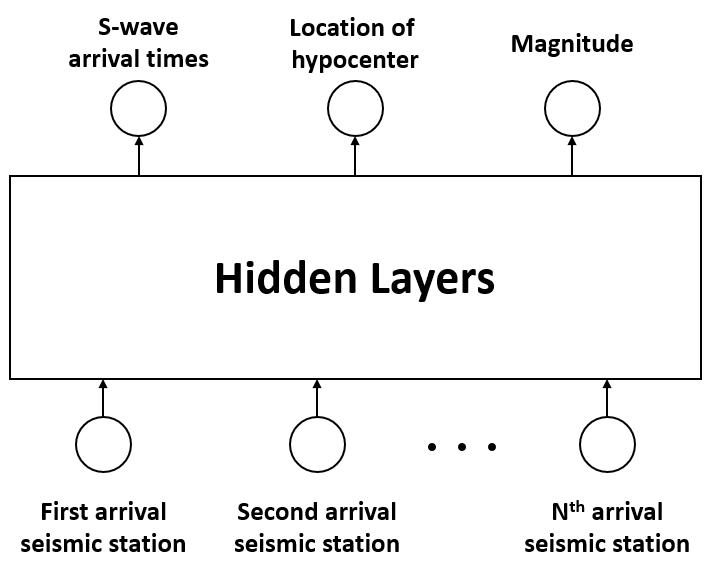
\includegraphics[width=0.48\textwidth]{figs/overview_model.png}
\caption{Overview of DNN model}
\label{fig:overview_model}
\end{figure}

The model uses input features as latitude and longitude of seismic stations and arrival times of P-wave which is encoded in various formats. We use three loss functions to train our model. It is called multitask learning \cite{baxter1995learning} which prevents overfitting problem by designing a model to estimate various related tasks at once.

The model predicts three components. First, it estimates the arrival times of S-wave for each seismic station. It uses average of absolute difference of S-wave arrival time as a loss to train the model. The model optimizes (minimizes) the loss with ADADELTA \cite{zeiler2012adadelta} optimizer.

Second, it finds the epicenter and depth of the hypocenter. It uses mean squared error of latitude, longitude and depth to calculate the loss. The function simply emulate the difference of distance between hypocenter and predicted hypocenter. The model optimizes (minimizes) the loss with ADADELTA optimizer.

Third, it predicts magnitude of the earthquake. It uses absolute difference of magnitude for the loss function. The model optimizes (minimizes) the loss with ADADELTA optimizer.
